\documentclass[tikz,border=5pt]{standalone}
\usepackage{tikz}
\usetikzlibrary{arrows.meta,positioning,matrix}

\begin{document}
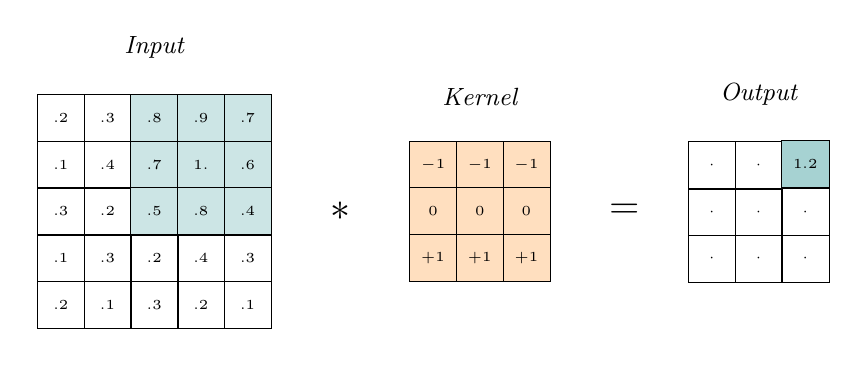
\begin{tikzpicture}[
    cell/.style={minimum size=0.6cm, draw, very thin, font=\tiny},
    highlight/.style={cell, fill=teal!20},
    kernel/.style={cell, fill=orange!25},
    outcell/.style={cell, fill=teal!35},
    arrow/.style={-{Stealth[length=2mm]}, thick},
    label/.style={font=\small\itshape}
]

% Input image (5x5)
\matrix (input) [matrix of nodes, nodes={cell}, column sep=-\pgflinewidth, row sep=-\pgflinewidth] {
    .2 & .3 & |[highlight]| .8 & |[highlight]| .9 & |[highlight]| .7 \\
    .1 & .4 & |[highlight]| .7 & |[highlight]| 1. & |[highlight]| .6 \\
    .3 & .2 & |[highlight]| .5 & |[highlight]| .8 & |[highlight]| .4 \\
    .1 & .3 & .2 & .4 & .3 \\
    .2 & .1 & .3 & .2 & .1 \\
};

% Kernel (3x3)
\matrix (kernel) [matrix of nodes, nodes={kernel}, column sep=-\pgflinewidth, row sep=-\pgflinewidth, right=1.5cm of input] {
    $-1$ & $-1$ & $-1$ \\
    $0$ & $0$ & $0$ \\
    $+1$ & $+1$ & $+1$ \\
};

% Output (3x3)
\matrix (output) [matrix of nodes, nodes={cell}, column sep=-\pgflinewidth, row sep=-\pgflinewidth, right=1.5cm of kernel] {
    $\cdot$ & $\cdot$ & |[outcell]| 1.2 \\
    $\cdot$ & $\cdot$ & $\cdot$ \\
    $\cdot$ & $\cdot$ & $\cdot$ \\
};

% Operators
\node[right=0.5cm of input, font=\Large] {$*$};
\node[right=0.5cm of kernel, font=\Large] {$=$};

% Labels
\node[above=0.2cm of input, label] {Input};
\node[above=0.2cm of kernel, label] {Kernel};
\node[above=0.2cm of output, label] {Output};

\end{tikzpicture}
\end{document}
